\section{系统设计}

\subsection{系统数据流图}

在设计本系统时,面临着多个关键挑战:首先是需要处理来自不同招聘网站的异构数据,这些数据格式和结构各不相同;其次是需要确保数据的实时性和准确性,因为招聘信息经常会发生变化;最后是需要提供高效的数据查询和分析功能,以支持各种数据可视化和统计分析需求。

为了应对这些挑战,采用了分层架构设计,通过清晰的数据流向和模块划分,实现了从数据采集到数据展示的完整流程。如图\ref{fig:system_dataflow_simplified}所示,系统主要包含六个核心层次:外部数据源层、ETL处理层、数据存储层、CRUD层、API服务层和后台服务层。这种分层设计不仅使系统结构清晰,便于维护和扩展,还能够有效地隔离不同功能模块,提高系统的可靠性和可维护性。

\begin{figure}[htbp]
    \centering
    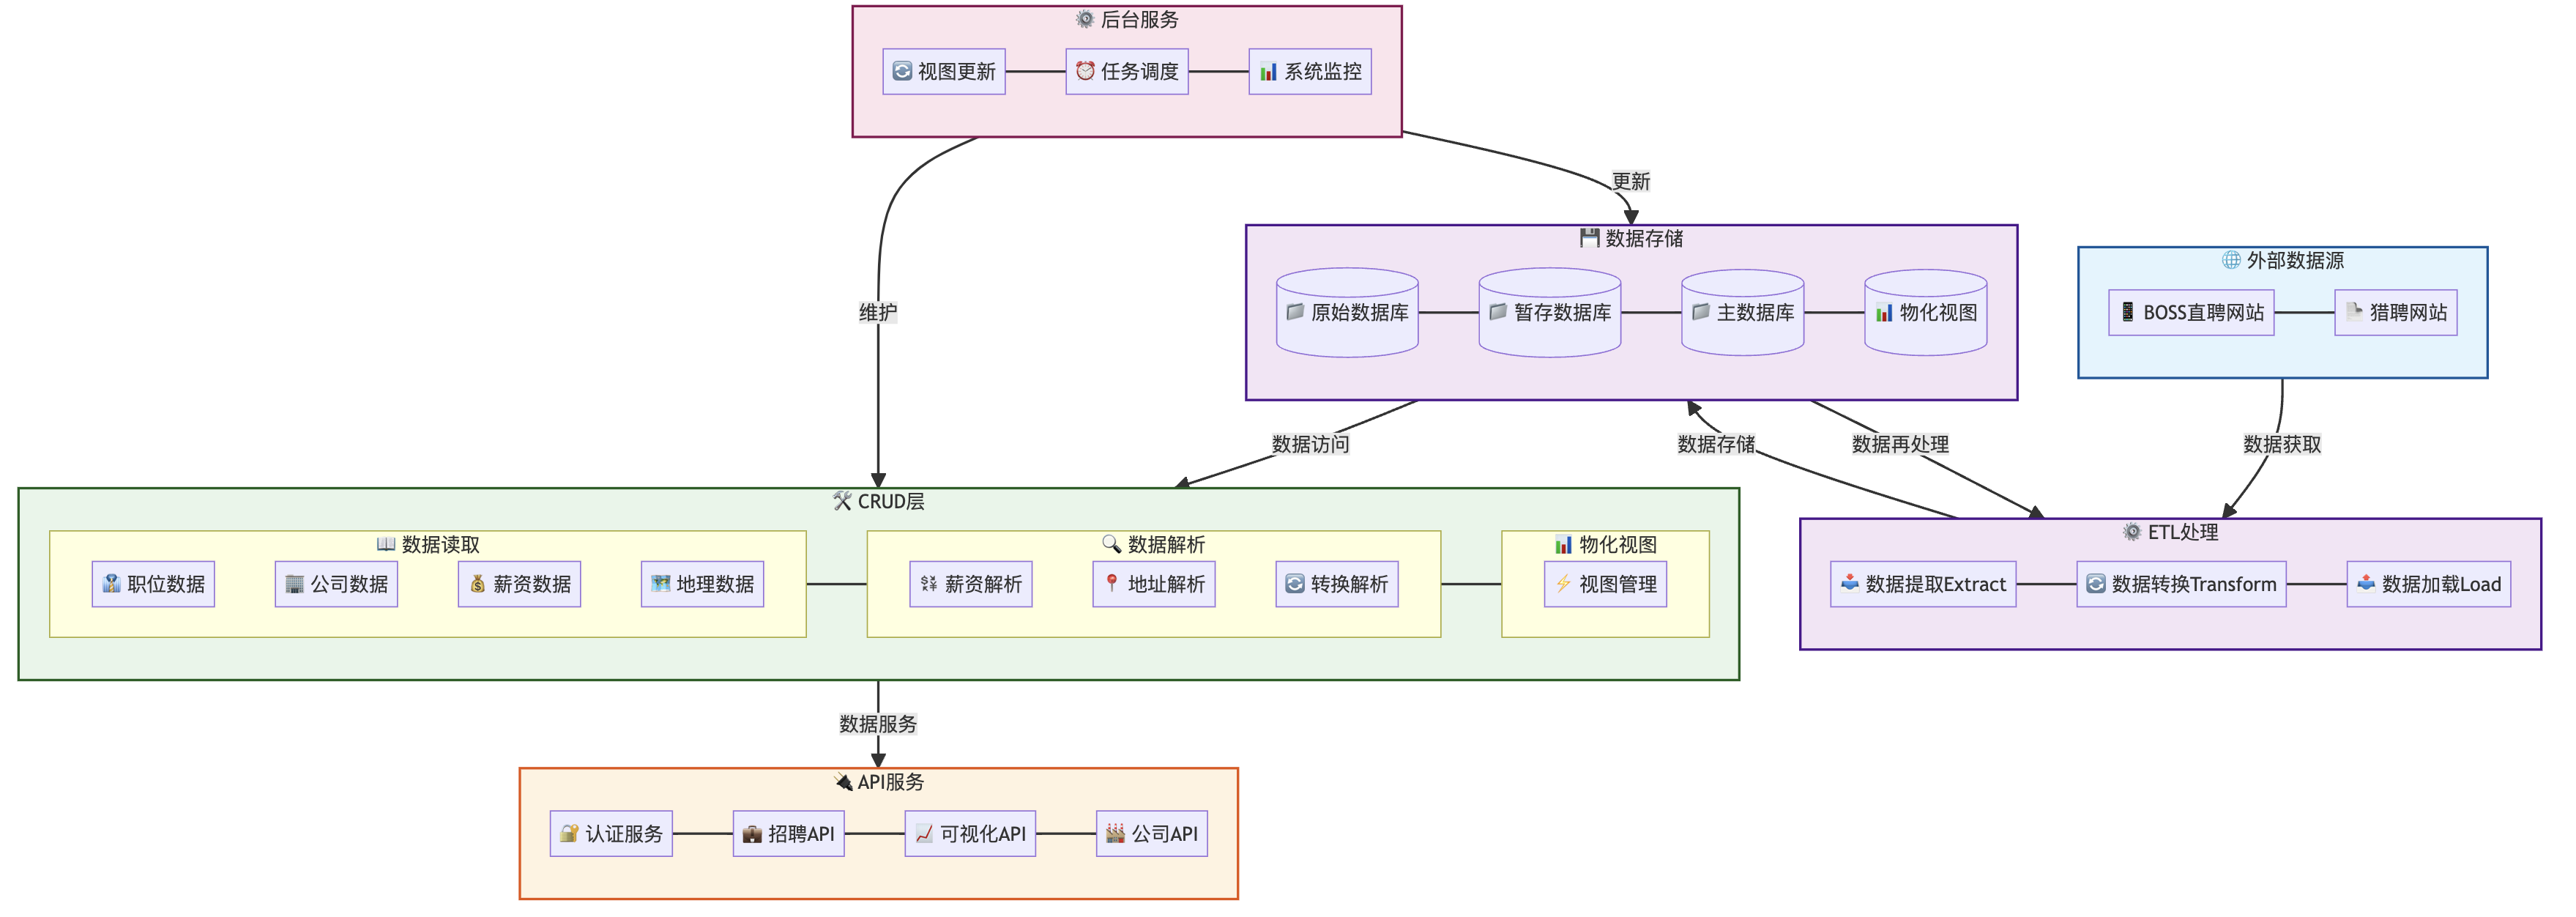
\includegraphics[width=1.0\textwidth]{figures/系统数据流图简化版.png}
    \caption{系统数据流图简化版}
    \label{fig:system_dataflow_simplified}
\end{figure}



图\ref{fig:system_dataflow}是系统数据流图的详细版本,展示了系统从数据采集到数据展示的完整流程。该图通过流程图的形式详细展示了系统的数据流向:从BOSS直聘和猎聘网站的数据源开始,数据首先经过ETL处理层的提取、转换和加载三个阶段,然后依次存储在原始数据库、暂存数据库、主数据库和物化视图中。CRUD层负责数据的基础操作,包括职位、公司、薪资和地理数据的读取与解析,以及物化视图的管理。API服务层则提供了认证、招聘信息、可视化和公司信息等对外接口。整个系统由后台服务层的任务调度器进行统一调度,通过物化视图更新服务保持数据的实时性,并通过系统监控确保各个模块的正常运行。这种层次分明的架构设计不仅确保了数据处理的完整性和可靠性,也为系统的扩展和维护提供了便利。

\begin{figure}[htbp]
    \centering
    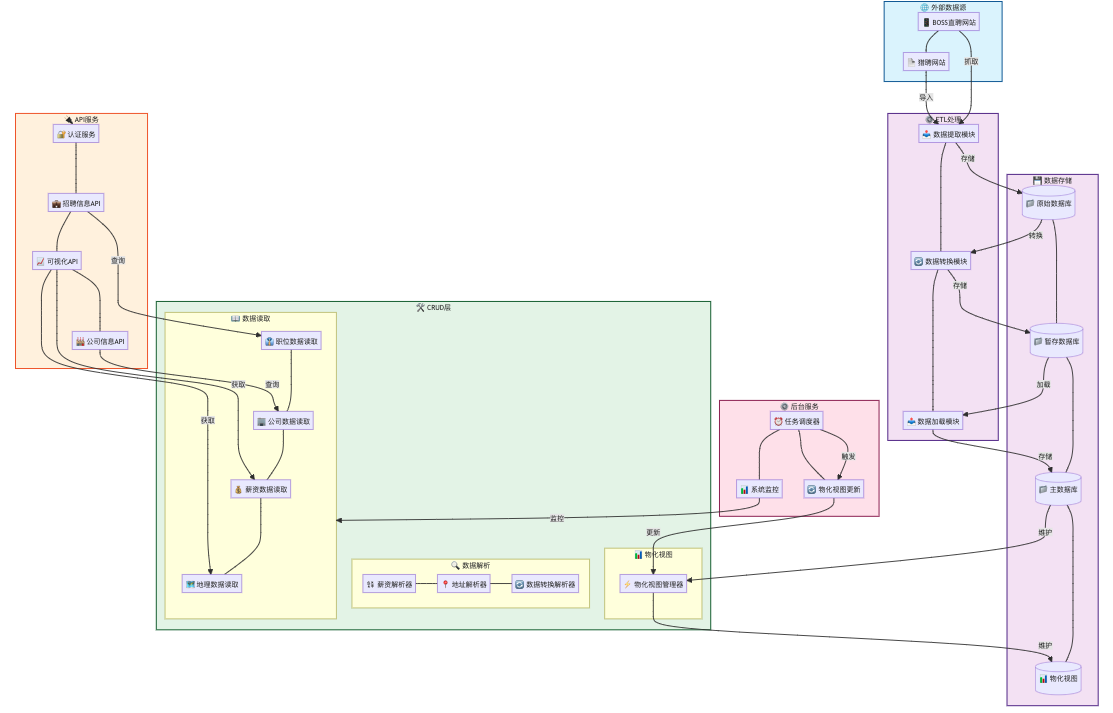
\includegraphics[width=1.0\textwidth]{figures/系统数据流图.png}
    \caption{系统数据流图}
    \label{fig:system_dataflow}
\end{figure}

\subsection{数据集成}
本系统实现了一个完整的ETL(Extract-Transform-Load)数据集成流程,将来自不同招聘网站的职位数据进行整合、清洗和标准化,最终加载到规范化的数据库中。整个过程包括数据抽取(Extract)、数据转换(Transform)和数据加载(Load)三个主要阶段。如图\ref{fig:ETL}所示。

\begin{figure}[htbp]
    \centering
    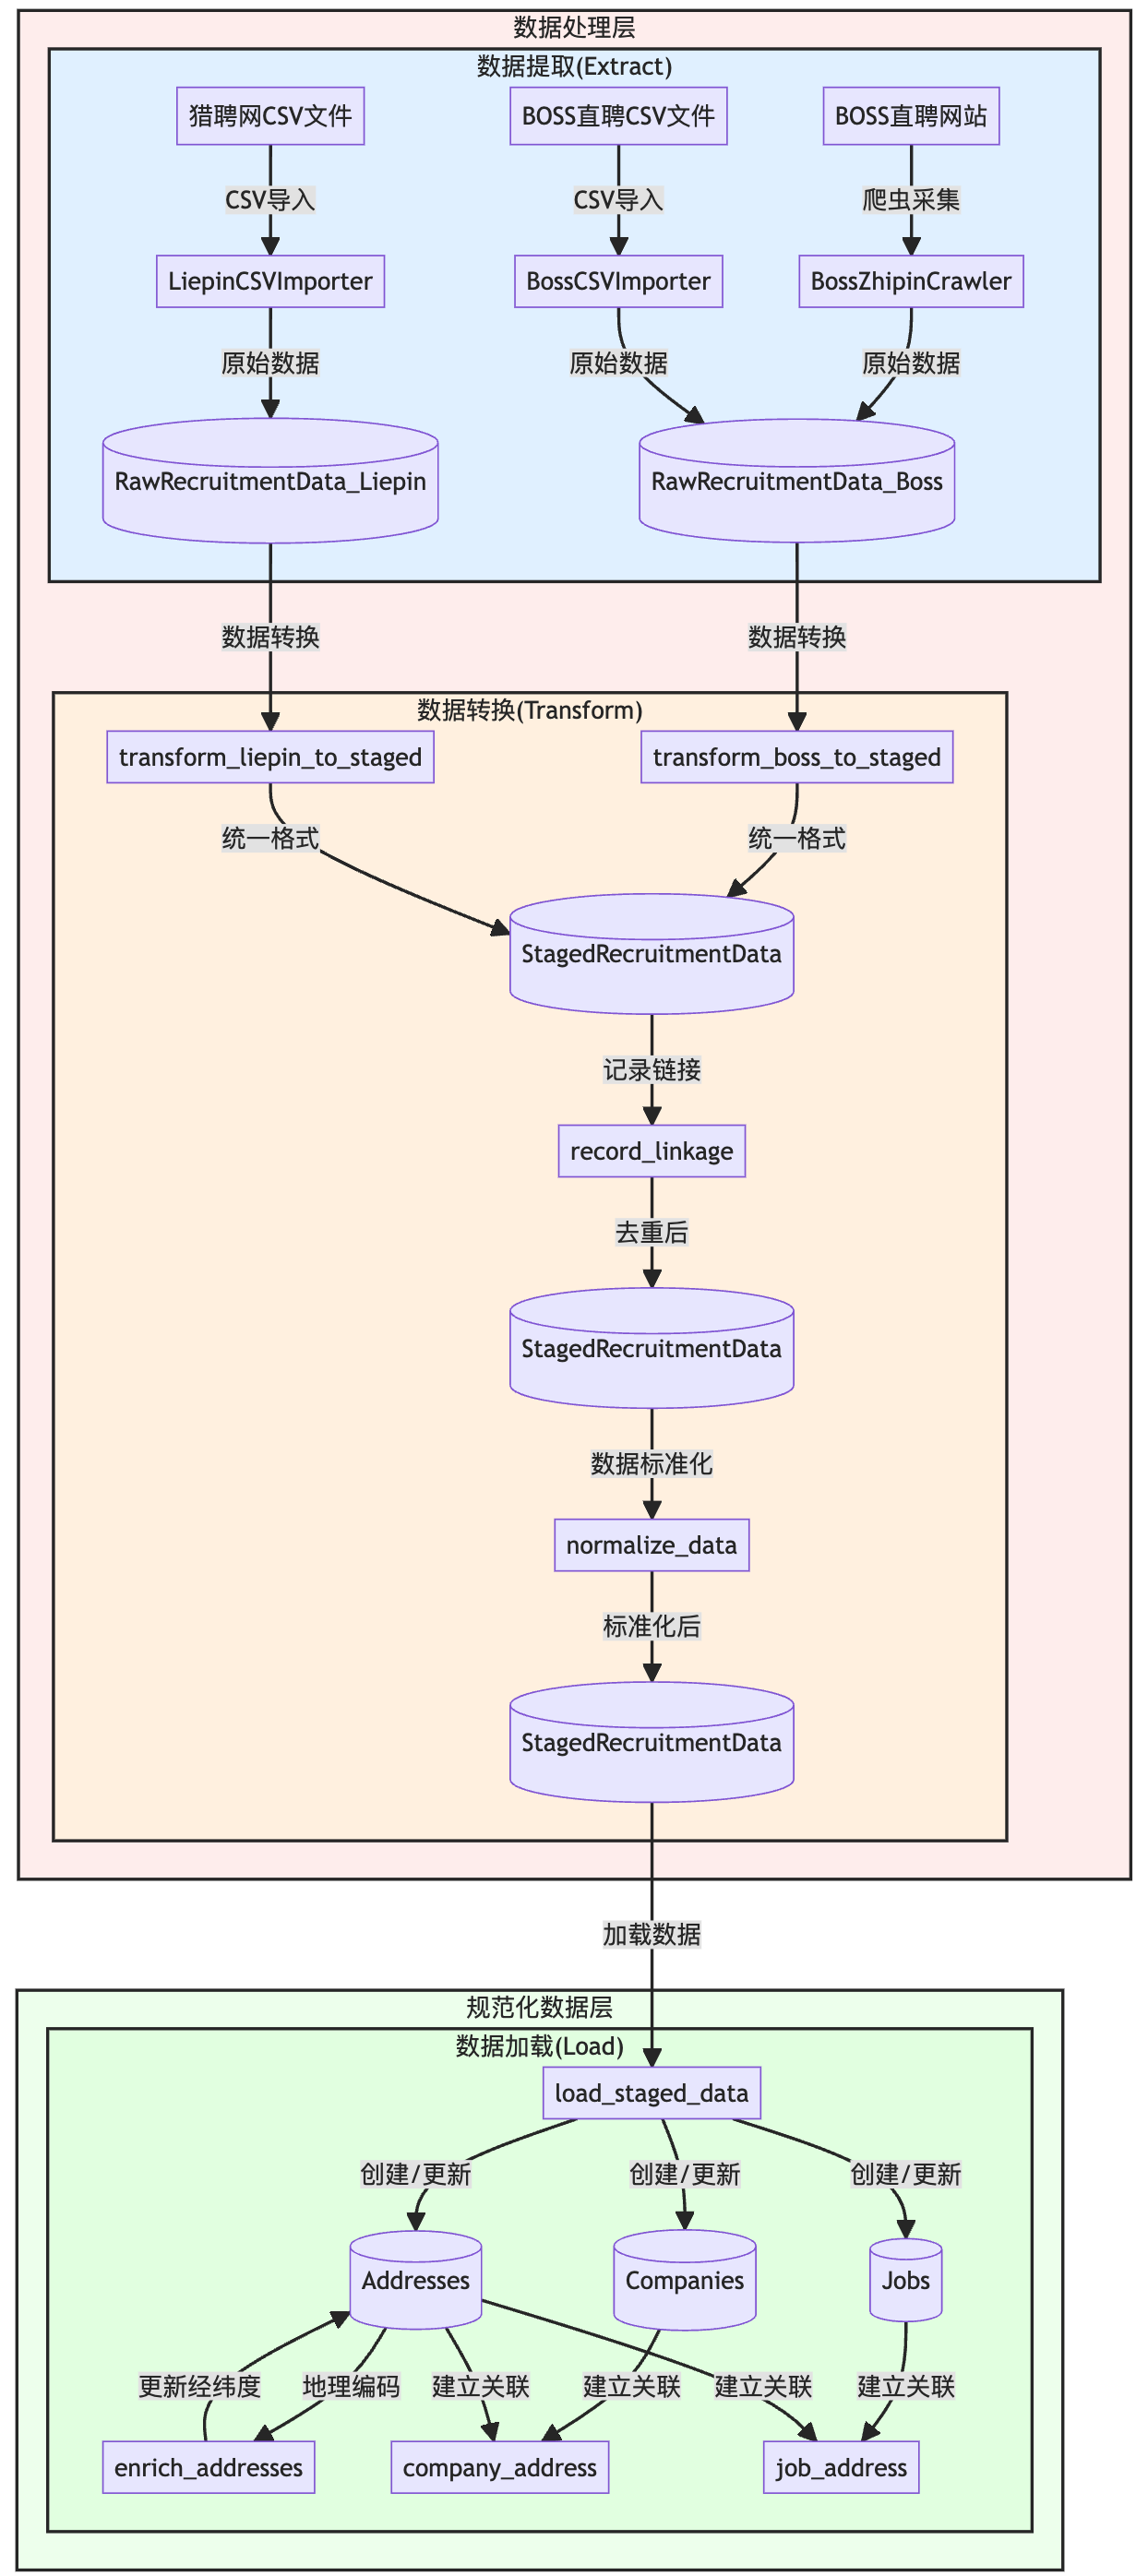
\includegraphics[width=0.6\textwidth]{figures/ETL.png}
    \caption{ETL数据集成流程}
    \label{fig:ETL}
\end{figure}

\subsubsection{数据抽取(Extract)}
数据抽取阶段主要通过两种方式获取数据,如图\ref{fig:ETL_extract}所示。包含下面两个步骤:

\begin{figure}[htbp]
    \centering
    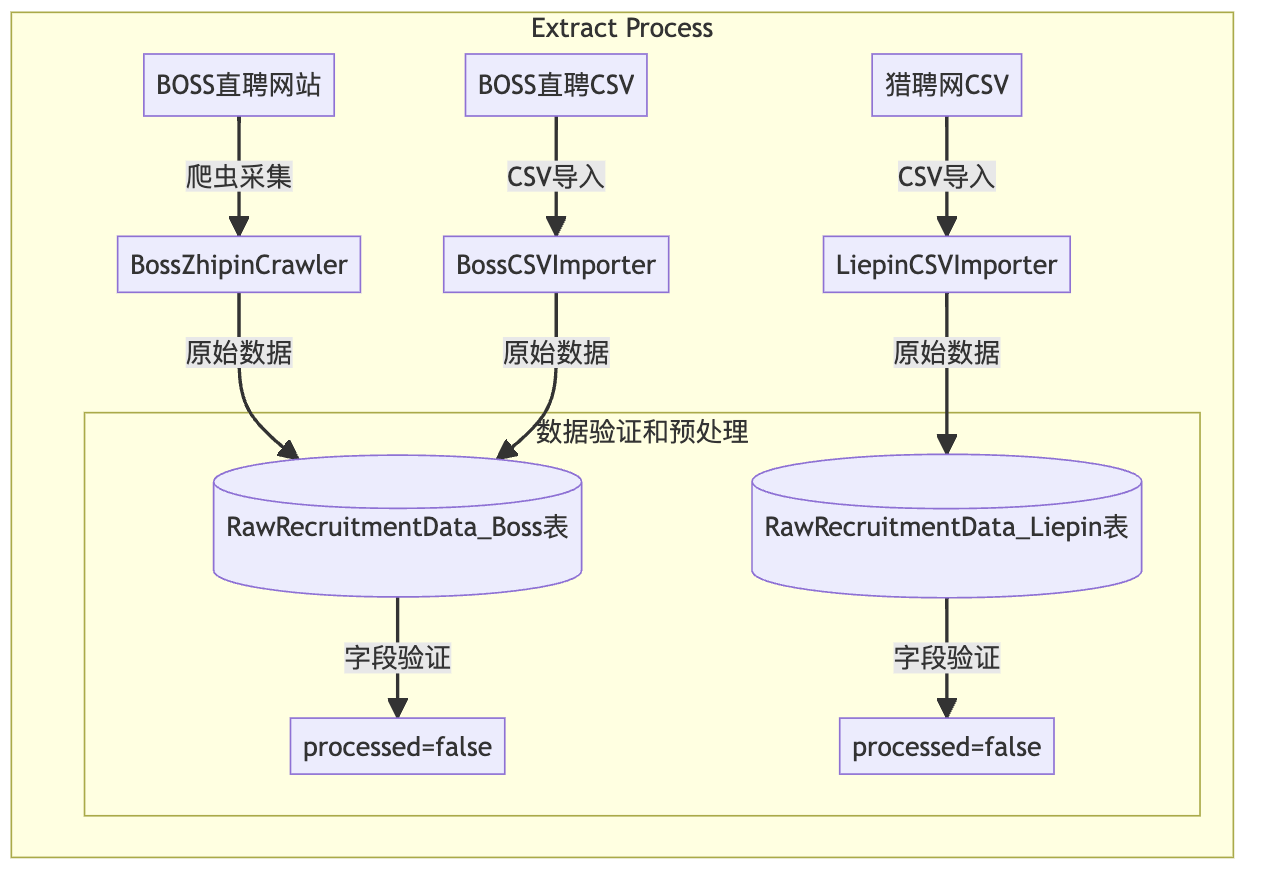
\includegraphics[width=0.5\textwidth]{figures/extract.png}
    \caption{数据抽取流程}
    \label{fig:ETL_extract}
\end{figure}


\begin{itemize}
    \item \textbf{Boss直聘数据抽取}:
    \begin{itemize}
        \item 使用Selenium实现网页爬虫,支持自动翻页和错误重试
        \item 提取职位信息、公司信息、地址等数据
        \item 数据直接存入raw\_recruitment\_boss表
    \end{itemize}
    
    \item \textbf{猎聘网数据导入}:
    \begin{itemize}
        \item 通过CSV文件导入,支持批量处理和数据验证
        \item 数据存入raw\_recruitment\_liepin表
    \end{itemize}
\end{itemize}

\subsubsection{数据转换(Transform)}
数据转换阶段是整个ETL过程中最复杂的部分,主要包括以下几个关键步骤,如图\ref{fig:ETL_transform}所示。

\begin{figure}[htbp]
    \centering
    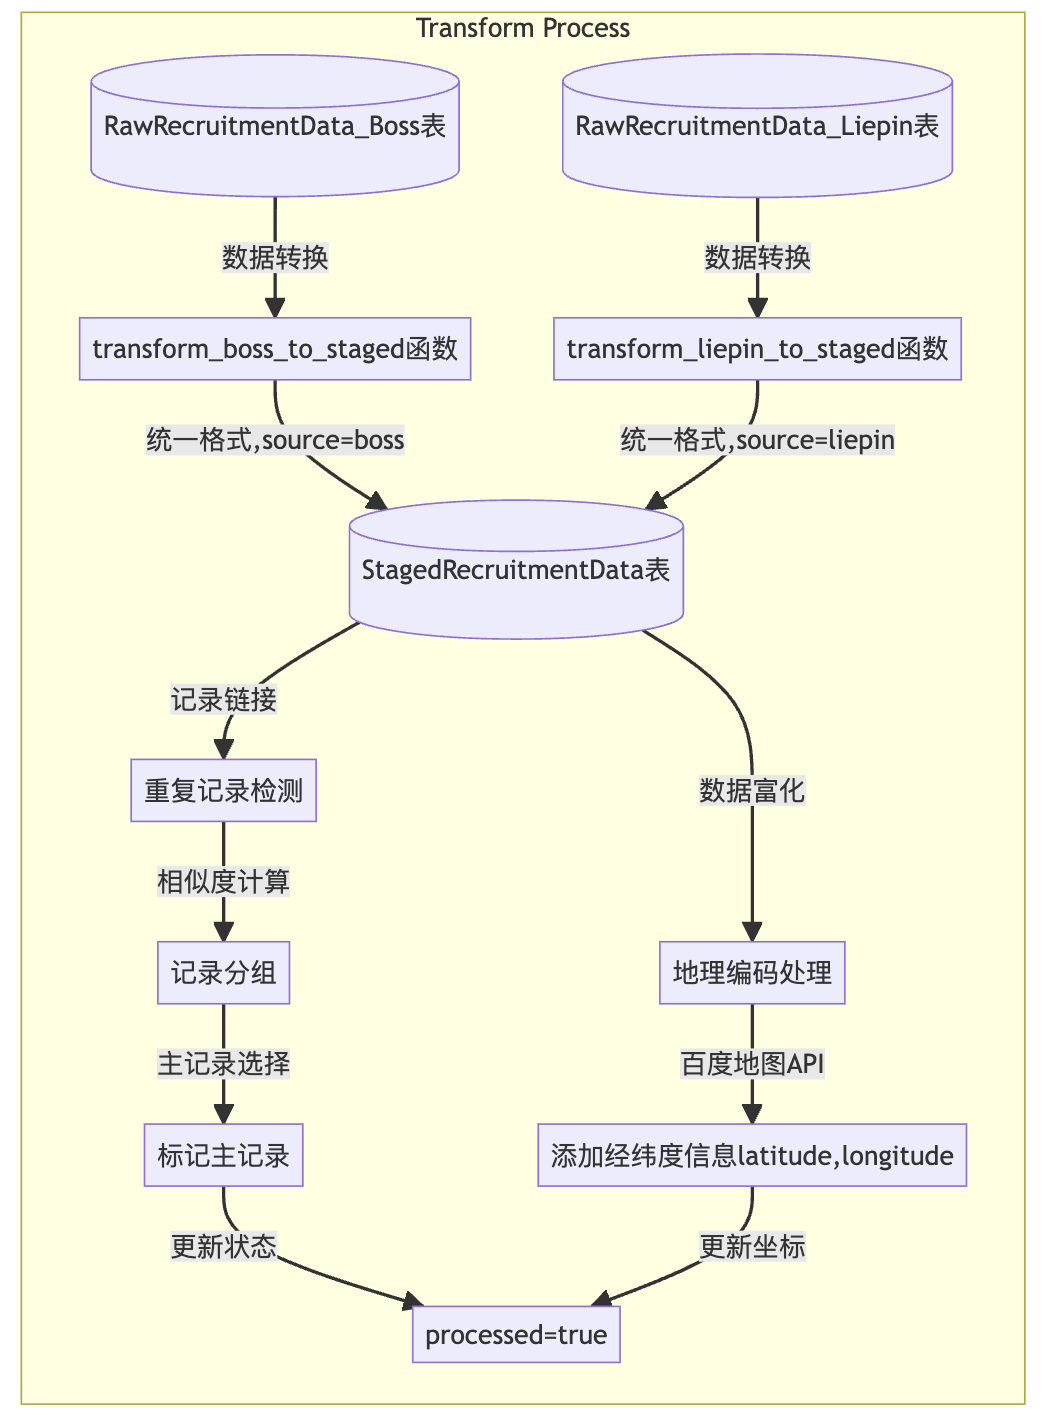
\includegraphics[width=0.5\textwidth]{figures/transform.png}
    \caption{数据转换流程}
    \label{fig:ETL_transform}
\end{figure}

数据转换过程主要包括三个部分:Boss直聘数据转换、猎聘网数据转换以及额外字段转换。如图\ref{fig:boss_transform}、图\ref{fig:liepin_transform}和图\ref{fig:extra_transform}所示。

\begin{figure}[htbp]
    \centering
    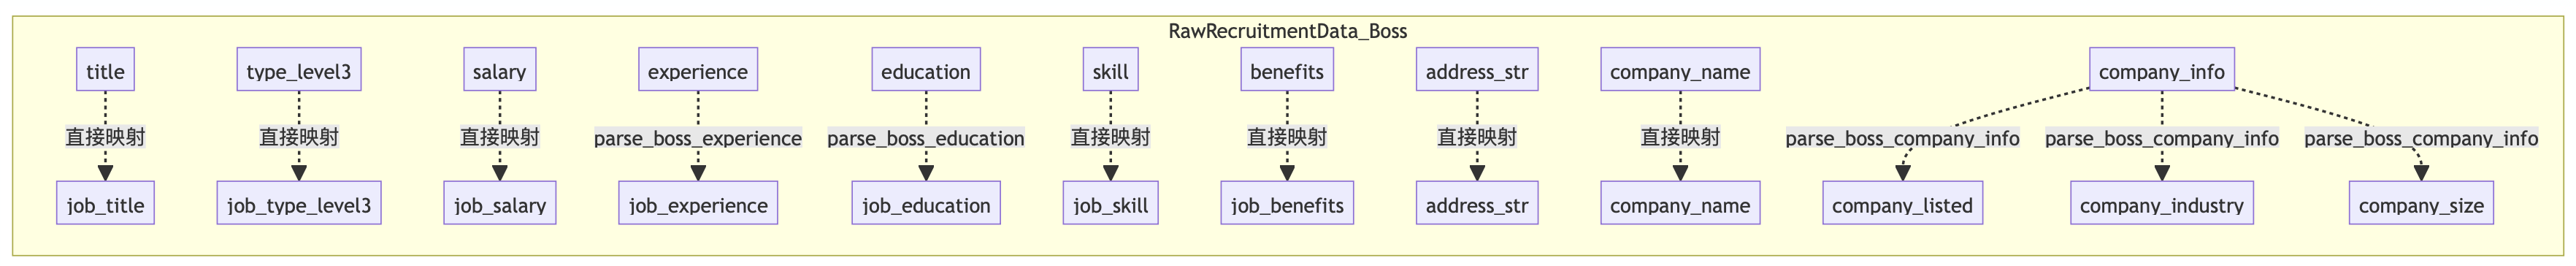
\includegraphics[width=1.0\textwidth]{figures/T过程boss.png}
    \caption{Boss直聘数据转换流程}
    \label{fig:boss_transform}
\end{figure}

从图\ref{fig:boss_transform}可以看出,Boss直聘数据的转换过程主要包括直接映射和解析转换两种方式。其中title、type\_level3、salary等字段可以直接映射到目标表,而experience、education和company\_info等字段则需要通过特定的解析函数进行转换。

\begin{figure}[htbp]
    \centering
    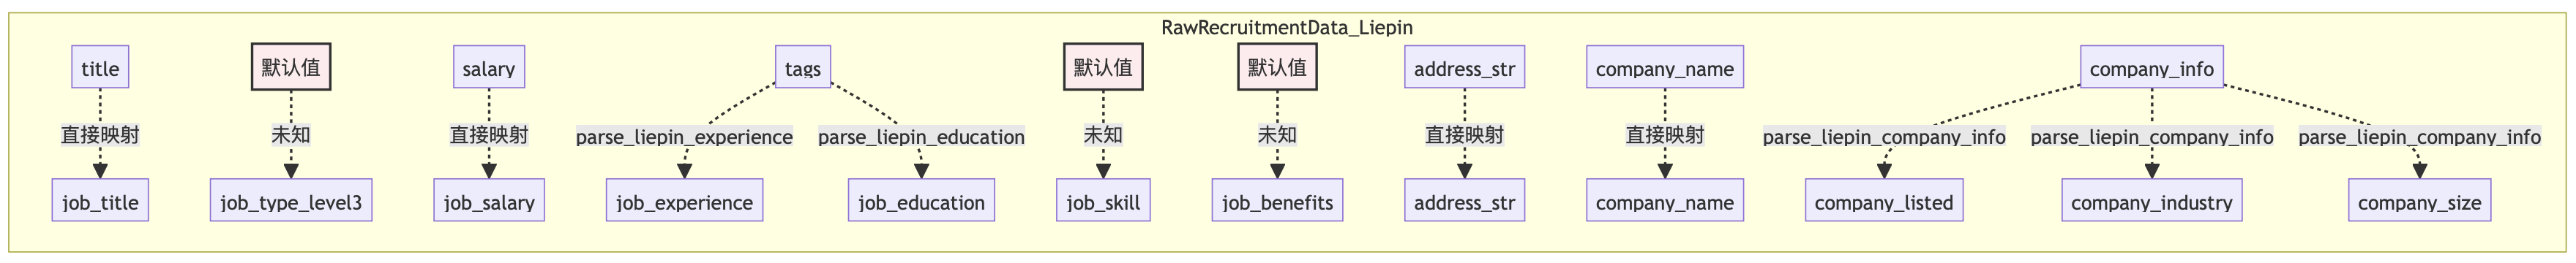
\includegraphics[width=1.0\textwidth]{figures/T过程liepin.png}
    \caption{猎聘网数据转换流程}
    \label{fig:liepin_transform}
\end{figure}

图\ref{fig:liepin_transform}展示了猎聘网数据的转换流程。由于猎聘网的数据结构与Boss直聘不同,需要针对其特有的tags字段进行解析,从中提取职位类型、工作经验、教育要求等信息。

\begin{figure}[htbp]
    \centering
    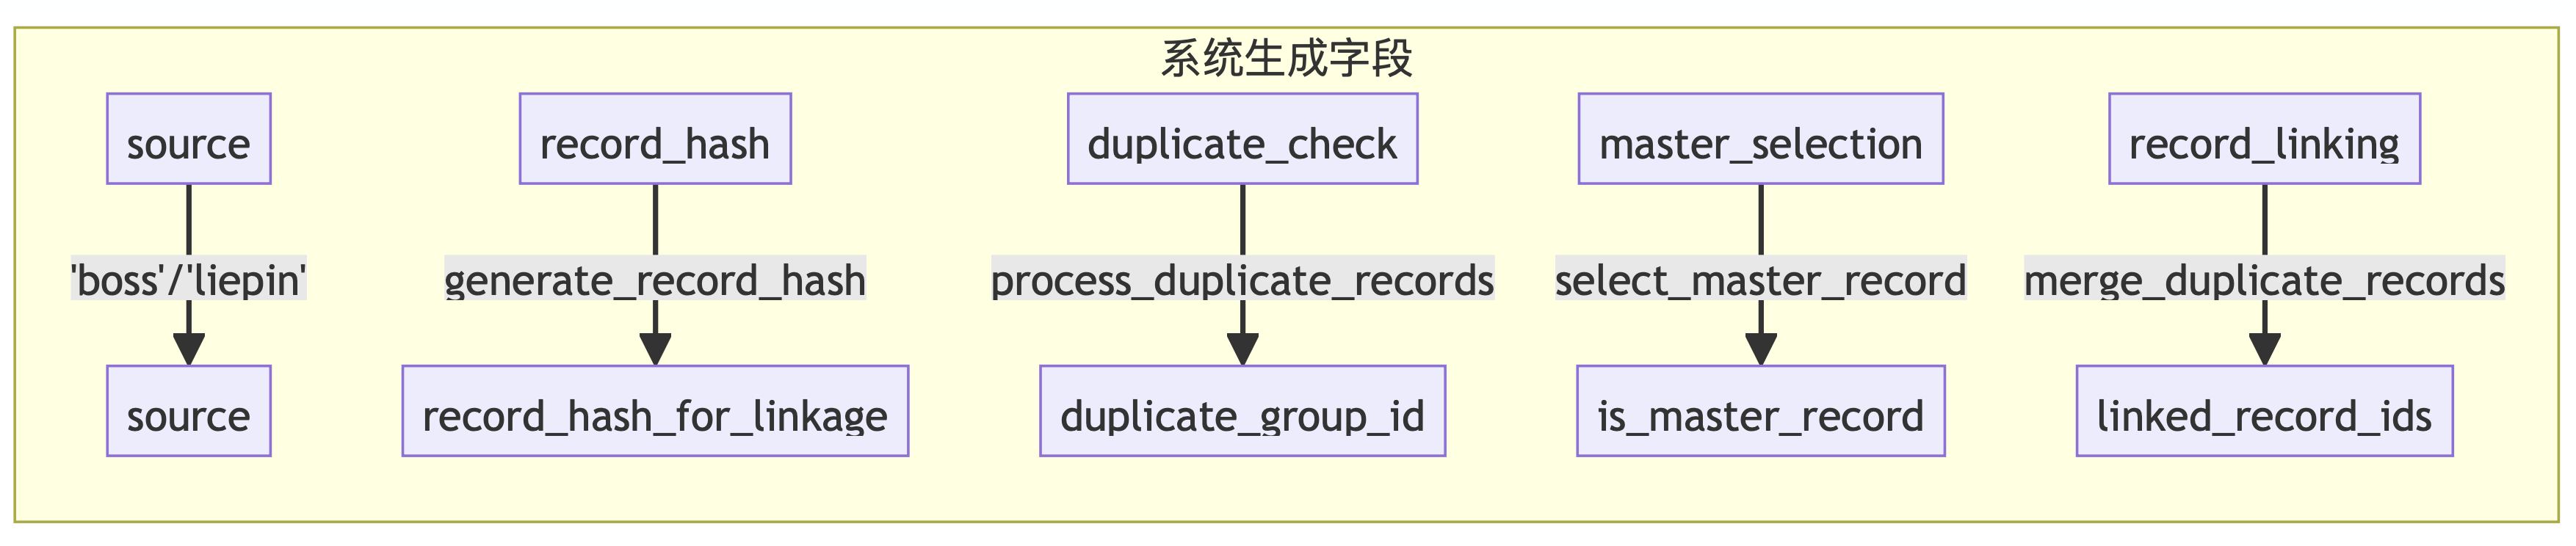
\includegraphics[width=1\textwidth]{figures/T过程extra.png}
    \caption{额外字段转换流程}
    \label{fig:extra_transform}
\end{figure}

图\ref{fig:extra_transform}显示了一些需要额外处理的字段转换过程,包括record\_hash\_for\_linkage的生成、duplicate\_group\_id的分配以及is\_master\_record的判定等。这些字段主要用于后续的记录链接和去重处理。

这个过程可以总结如下:

\begin{itemize}
    \item \textbf{数据清洗和标准化}:
    \begin{itemize}
        \item 实现了文本预处理和标准化
        \item 去除空白字符、转换英文字符为小写
        \item 移除标点符号,保留中文和英文字符
    \end{itemize}
    
    \item \textbf{记录链接和去重}:
    \begin{itemize}
        \item 采用多阶段策略进行记录链接
        \item 使用特征提取和哈希生成进行快速初筛
        \item 通过Jaccard相似度算法计算文本相似度
        \item 动态权重分配,重点关注公司名称和职位名称
    \end{itemize}
    
    \item \textbf{数据融合策略}:
    \begin{itemize}
        \item 智能选择主记录(基于记录完整度)
        \item 维护重复记录之间的关联关系
        \item 支持增量更新和批量处理
    \end{itemize}
\end{itemize}

\subsubsection{数据加载(Load)}

数据加载阶段是ETL过程的最后一个环节,负责将暂存表中的数据规范化加载到最终的数据库中。在这个阶段,系统首先会对数据进行全面的验证和预处理,包括检查必要字段的完整性、验证数据格式的正确性,以及进行必要的数据类型转换。这一步骤确保了进入最终数据库的数据都是高质量且格式统一的。

在数据验证完成后,系统会进行地理编码处理。这个过程通过调用百度地图API,将地址字符串转换为具体的经纬度坐标。系统采用了批量处理的方式提高效率,同时实现了错误重试机制以提高地理编码的成功率。对于无法成功编码的地址,系统会记录详细的错误信息,便于后续人工处理或重试。

最后是数据的规范化加载过程。这个阶段系统会根据数据库的规范化设计,将数据分别加载到不同的实体表中。首先是创建或更新公司信息,系统会检查公司是否已存在,如果存在则更新相关信息,如果不存在则创建新的公司记录。然后是处理地址信息,由于一个公司可能有多个地址,系统支持多地址的处理和存储。接着是创建职位记录,将职位相关的所有信息存入职位表中。最后,系统会建立各个实体之间的关联关系,包括公司与地址之间的关系、职位与地址之间的关系等。整个加载过程采用事务管理机制,确保数据的一致性和完整性。

为了提高数据加载的效率,系统采用了批量处理的策略,同时实现了完善的错误处理机制。当加载过程中出现异常时,系统会自动回滚事务,确保数据库的一致性不被破坏。同时,系统会详细记录每一步的处理结果,包括成功加载的记录数、失败的记录数以及具体的错误原因,这些信息对于后续的数据质量分析和系统优化都有重要的参考价值。

整个过程如图\ref{fig:ETL_load}所示。

\begin{figure}[htbp]
    \centering
    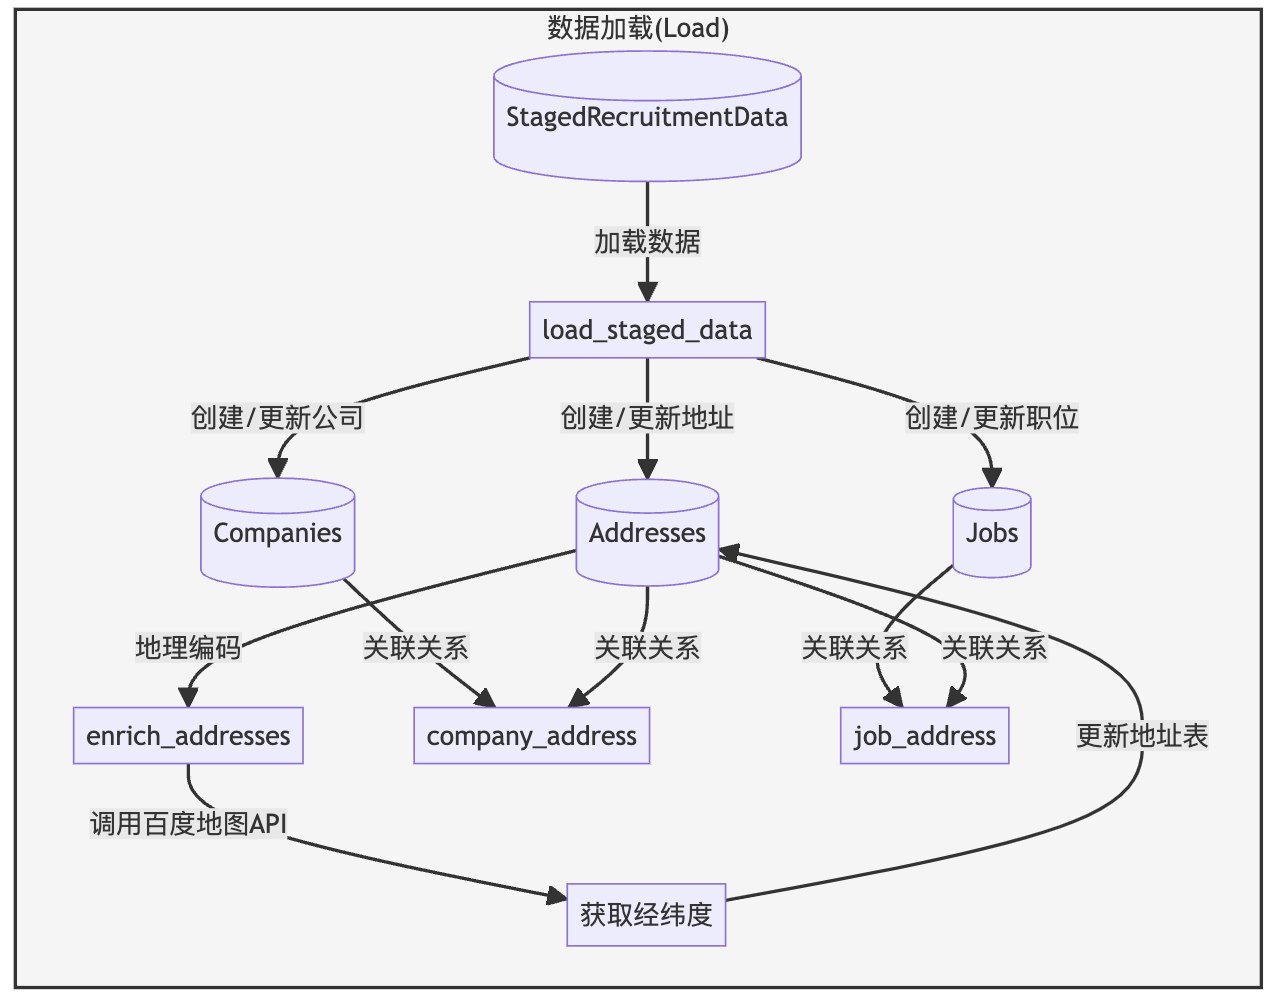
\includegraphics[width=0.5\textwidth]{figures/load.png}
    \caption{ETL数据加载流程}
    \label{fig:ETL_load}
\end{figure}

\subsubsection{CRUD层}
CRUD层作为系统的数据访问中间层,提供了统一的数据操作接口。该层的设计遵循了领域驱动设计(DDD)的原则,将业务逻辑与数据访问清晰分离:

\begin{itemize}
    \item \textbf{数据读取模块}:
    \begin{itemize}
        \item 职位数据读取:实现了高效的职位信息检索,支持多条件组合查询
        \item 公司数据读取:提供完整的公司信息访问接口,支持模糊匹配和精确查询
        \item 薪资数据读取:实现了复杂的薪资统计算法,支持多维度的薪资分析
        \item 地理数据读取:提供基于地理位置的数据检索,支持范围查询和距离计算
    \end{itemize}
    
    \item \textbf{数据解析模块}:
    \begin{itemize}
        \item 薪资解析器:采用智能算法解析多种格式的薪资描述,实现标准化处理
        \item 地址解析器:结合百度地图API,实现精确的地址解析和地理编码
        \item 数据转换解析器:提供灵活的数据转换框架,支持自定义转换规则
    \end{itemize}
    
    \item \textbf{物化视图管理}:
    \begin{itemize}
        \item 实现了智能的视图更新策略,根据数据变化频率动态调整更新周期
        \item 提供了完整的视图管理接口,支持视图的创建、更新和删除
        \item 实现了视图依赖管理,确保相关视图的同步更新
    \end{itemize}
\end{itemize}
\subsubsection{后台服务层}
后台服务层负责系统的维护和监控工作,确保系统的稳定运行和数据的实时更新:

\begin{itemize}
    \item \textbf{物化视图更新}:
    \begin{itemize}
        \item 实现了基于时间触发的自动更新机制
        \item 支持手动触发的即时更新
        \item 提供了更新状态的监控接口
    \end{itemize}
    
    \item \textbf{任务调度器}:
    \begin{itemize}
        \item 基于APScheduler实现了灵活的任务调度系统
        \item 支持定时任务和周期性任务的管理
        \item 提供了任务执行状态的监控和告警
    \end{itemize}
    
    \item \textbf{系统监控}:
    \begin{itemize}
        \item 实现了全面的性能监控指标收集
        \item 提供了系统运行状态的实时监控
        \item 支持异常情况的自动告警
    \end{itemize}
\end{itemize}

\subsection{数据流向说明}
系统的数据流向设计充分考虑了数据处理的效率和可靠性,主要包括以下几个方面:

\begin{enumerate}
    \item \textbf{数据采集流向}:
    \begin{itemize}
        \item 外部数据源 → ETL处理层:通过爬虫采集数据,实现了自动化的数据获取过程
        \item ETL处理层 → 原始数据库:采用批量写入策略,确保数据采集的效率
    \end{itemize}
    
    \item \textbf{数据处理流向}:
    \begin{itemize}
        \item 原始数据库 → 数据转换模块:实现了增量数据处理,避免重复处理
        \item 数据转换模块 → 暂存数据库:采用事务处理,确保数据一致性
        \item 暂存数据库 → 数据加载模块:实现了智能的数据加载策略
        \item 数据加载模块 → 主数据库:通过批量操作优化性能
    \end{itemize}
    
    \item \textbf{数据访问流向}:
    \begin{itemize}
        \item 主数据库/物化视图 → CRUD层:实现了高效的数据访问机制
        \item CRUD层 → API服务层:提供了标准化的数据服务接口
    \end{itemize}
    
    \item \textbf{维护流向}:
    \begin{itemize}
        \item 后台服务 → 物化视图管理器:实现了智能的视图更新策略
        \item 后台服务 → 数据读取模块:提供了完整的监控和维护机制
    \end{itemize}
\end{enumerate}

这种分层的数据流设计不仅确保了系统的可维护性和扩展性,还通过物化视图和缓存机制优化了系统性能。每一层都有明确的职责划分,通过标准化的接口进行通信,这种设计极大地降低了系统的耦合度,提高了代码的可重用性。同时,完整的监控和维护机制确保了系统能够稳定可靠地运行,满足实际应用的需求。

\subsection{API实现}

系统的API层采用FastAPI框架实现,遵循RESTful架构设计原则,提供了一系列标准化的HTTP接口。API的实现主要分为以下几个模块:

\subsubsection{认证模块(/auth)}
认证模块负责用户的身份验证和授权管理:

\begin{itemize}
    \item \textbf{登录接口}:
    \begin{itemize}
        \item 路径:\texttt{/auth/login}
        \item 方法:POST
        \item 功能:验证用户身份并返回用户信息
        \item 实现:基于JWT的身份验证机制
    \end{itemize}
\end{itemize}

\subsubsection{任务管理模块(/tasks)}
任务管理模块负责系统中各种数据处理任务的管理和监控:

\begin{itemize}
    \item \textbf{任务状态查询}:
    \begin{itemize}
        \item 路径:\texttt{/tasks/status}
        \item 方法:GET
        \item 功能:获取指定任务的执行状态
    \end{itemize}
    
    \item \textbf{任务触发}:
    \begin{itemize}
        \item 路径:\texttt{/tasks/trigger/\{task\_name\}}
        \item 方法:POST
        \item 功能:手动触发指定的任务
    \end{itemize}
    
    \item \textbf{数据导入任务}:
    \begin{itemize}
        \item 路径:\texttt{/tasks/add-data/import-data-liepin-csv}
        \item 方法:POST
        \item 功能:导入猎聘网CSV数据
    \end{itemize}
    
    \item \textbf{数据处理任务}:
    \begin{itemize}
        \item 路径:\texttt{/tasks/add-data/process-data-boss}
        \item 方法:POST
        \item 功能:处理BOSS直聘原始数据
    \end{itemize}
    
    \item \textbf{地理编码任务}:
    \begin{itemize}
        \item 路径:\texttt{/tasks/add-data/encode-addresses}
        \item 方法:POST
        \item 功能:处理地址的地理编码
    \end{itemize}
\end{itemize}

\subsubsection{招聘信息模块(/recruitments)}
招聘信息模块提供职位相关的数据访问接口:

\begin{itemize}
    \item \textbf{职位列表查询}:
    \begin{itemize}
        \item 路径:\texttt{/recruitments/}
        \item 方法:GET
        \item 功能:支持分页、排序和过滤的职位信息查询
    \end{itemize}
    
    \item \textbf{职位详情查询}:
    \begin{itemize}
        \item 路径:\texttt{/recruitments/\{job\_id\}}
        \item 方法:GET
        \item 功能:获取指定职位的详细信息
    \end{itemize}
\end{itemize}

\subsubsection{公司信息模块(/companies)}
公司信息模块提供公司相关的数据访问接口:

\begin{itemize}
    \item \textbf{公司列表查询}:
    \begin{itemize}
        \item 路径:\texttt{/companies/}
        \item 方法:GET
        \item 功能:支持分页的公司信息查询
    \end{itemize}
    
    \item \textbf{公司详情查询}:
    \begin{itemize}
        \item 路径:\texttt{/companies/\{company\_id\}}
        \item 方法:GET
        \item 功能:获取指定公司的详细信息
    \end{itemize}
\end{itemize}

\subsubsection{可视化模块(/visualization)}
可视化模块提供各种数据分析和可视化接口,下面只给出部分接口的示例,完整接口请参考代码。如图\ref{fig:visualization_api}所示,可以看到后端fastapi的接口文档。

\begin{itemize}
    \item \textbf{薪资分布分析}:
    \begin{itemize}
        \item 路径:\texttt{/visualization/salary-distribution/\{salary\_type\}}
        \item 方法:GET
        \item 功能:获取不同类型的薪资分布数据
        \item 参数:支持平均薪资、最高薪资、最低薪资等类型
    \end{itemize}
    
    \item \textbf{职位分布分析}:
    \begin{itemize}
        \item 路径:\texttt{/visualization/job-title-distribution}
        \item 方法:GET
        \item 功能:获取职位名称的分布统计
    \end{itemize}
    
    \item \textbf{地理分布分析}:
    \begin{itemize}
        \item 路径:\texttt{/visualization/salary-heatmap}
        \item 方法:GET
        \item 功能:获取薪资的地理分布热力图
    \end{itemize}
    
    \item \textbf{教育经验分析}:
    \begin{itemize}
        \item 路径:\texttt{/visualization/education-experience-distribution}
        \item 方法:GET
        \item 功能:分析学历要求与经验要求的关系
    \end{itemize}
    
    \item \textbf{行业薪资分析}:
    \begin{itemize}
        \item 路径:\texttt{/visualization/industry-salary-stats}
        \item 方法:GET
        \item 功能:分析不同行业的薪资情况
        \item 参数:支持不同的排序方式和图表显示模式
    \end{itemize}
\end{itemize}

\begin{figure}[htbp]
    \centering
    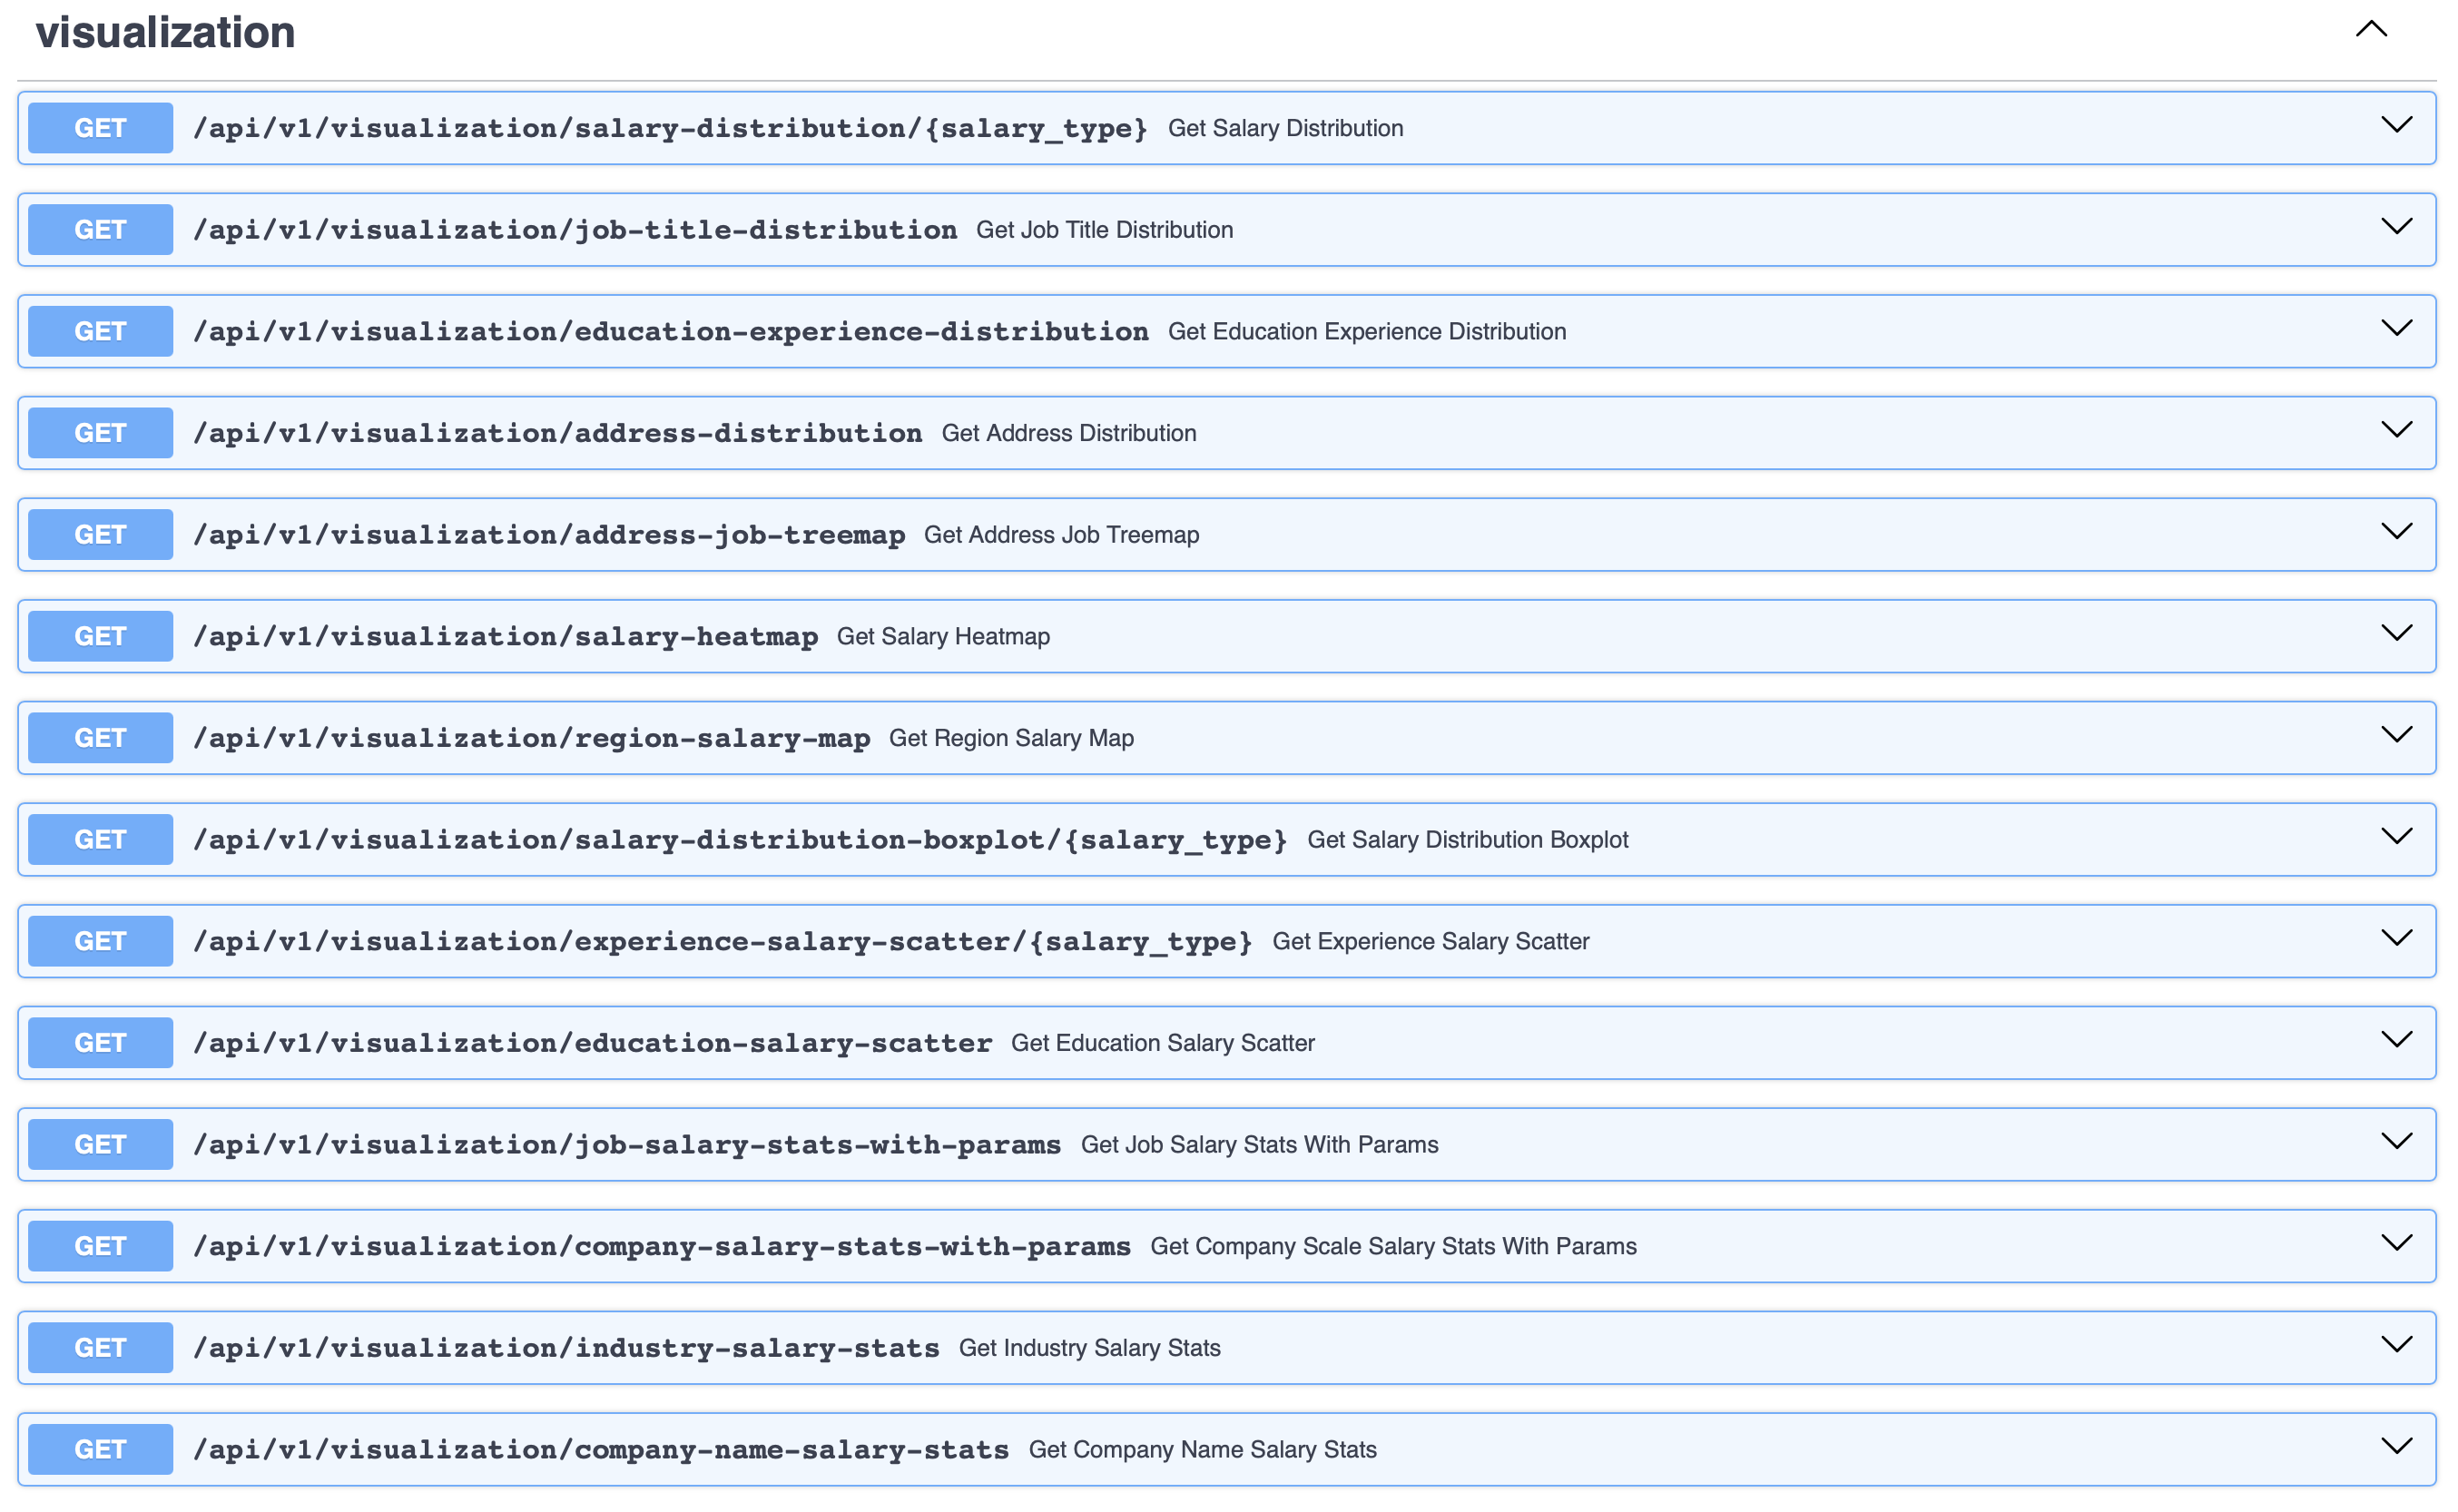
\includegraphics[width=0.9\textwidth]{figures/visualization_api.png}
    \caption{可视化模块API接口文档}
    \label{fig:visualization_api}
\end{figure}

\subsubsection{监控模块(/monitor)}
监控模块提供系统运行状态和数据质量的监控接口:

\begin{itemize}
    \item \textbf{数据质量监控}:
    \begin{itemize}
        \item 路径:\texttt{/monitor/data-quality}
        \item 方法:GET
        \item 功能:监控数据的完整性和质量
    \end{itemize}
    
    \item \textbf{数据一致性监控}:
    \begin{itemize}
        \item 路径:\texttt{/monitor/data-consistency}
        \item 方法:GET
        \item 功能:检查数据的一致性和完整性
    \end{itemize}
    
    \item \textbf{ETL进度监控}:
    \begin{itemize}
        \item 路径:\texttt{/monitor/etl-progress}
        \item 方法:GET
        \item 功能:监控ETL处理的进度
    \end{itemize}
    
    \item \textbf{系统性能监控}:
    \begin{itemize}
        \item 路径:\texttt{/monitor/system-performance}
        \item 方法:GET
        \item 功能:监控系统的性能指标
    \end{itemize}
\end{itemize}

